
\section{Experimental Results}
\label{s:evaluation}

Several experiments on various aspects of client-side anti-phishing indicate client-side classifier's inefficacious proficiency, insufficient features used in classifiers, ineffective server-side results, and the efficacy of content-based and real-time anti-phishing in desktop and mobile blacklisting.

\subsection{ Client-side classifier Detection Accuracy }
The classifier's result for 100 phishing websites shows that chrome client-side content-based anti-phishing could not detect 85\%  of phishing websites. This experiment signifies that the classifier has remarkable False Negative results. 
\begin{table}[]
\scalebox{0.8}{
\begin{tabular}{|c|c|c|}
\hline
\begin{tabular}[c]{@{}c@{}}Number of \\ Phishing websites\end{tabular} &
  \begin{tabular}[c]{@{}c@{}}Client-side classifier\\  result\end{tabular} &
  \begin{tabular}[c]{@{}c@{}}Sever-Side classifier\\  result\end{tabular} \\ \hline
100 &
  15\% &
  7\% \\ \hline
\end{tabular}%
}
\caption{Client-side and server-side detection ratio}
\label{tab: Client -side and server-side}
\end{table}

After our first experiment and the continuous dynamic analysis of chromium, we realized that the google safe browsing client-side phishing detection model has changed. 
Table \ref{ModelDifference} shows the difference between the new model and the old model. One of the most important changes in the new model is tuning the threshold.
Client-side anti-phishing detection does not use a static threshold ( which was 0.5) to identify the phishing sites. In the new model, google safe browsing tunes the threshold and send a dynamic threshold to the client. 
We confirm that classifier sets the threshold in function~\textit{threshold-probability()} which is a method of the \textit{Scorer} class defined in the file \textit{scorer.cc}. 
Figure \ref{fig:two model} shows the classifier's results with the old model and new model results. Although the scorer results are mainly changed, the dynamic threshold (During our experiment in late September, the model threshold was 0.88) became larger than the old static threshold(0.5). Therefore, the number of sites with the phishy score ( scores higher than the threshold) is noticeably low.
As shown in figure \ref{fig:two model} accuracy in the new model is improves by 35\%. 

 \begin{figure}
\centering
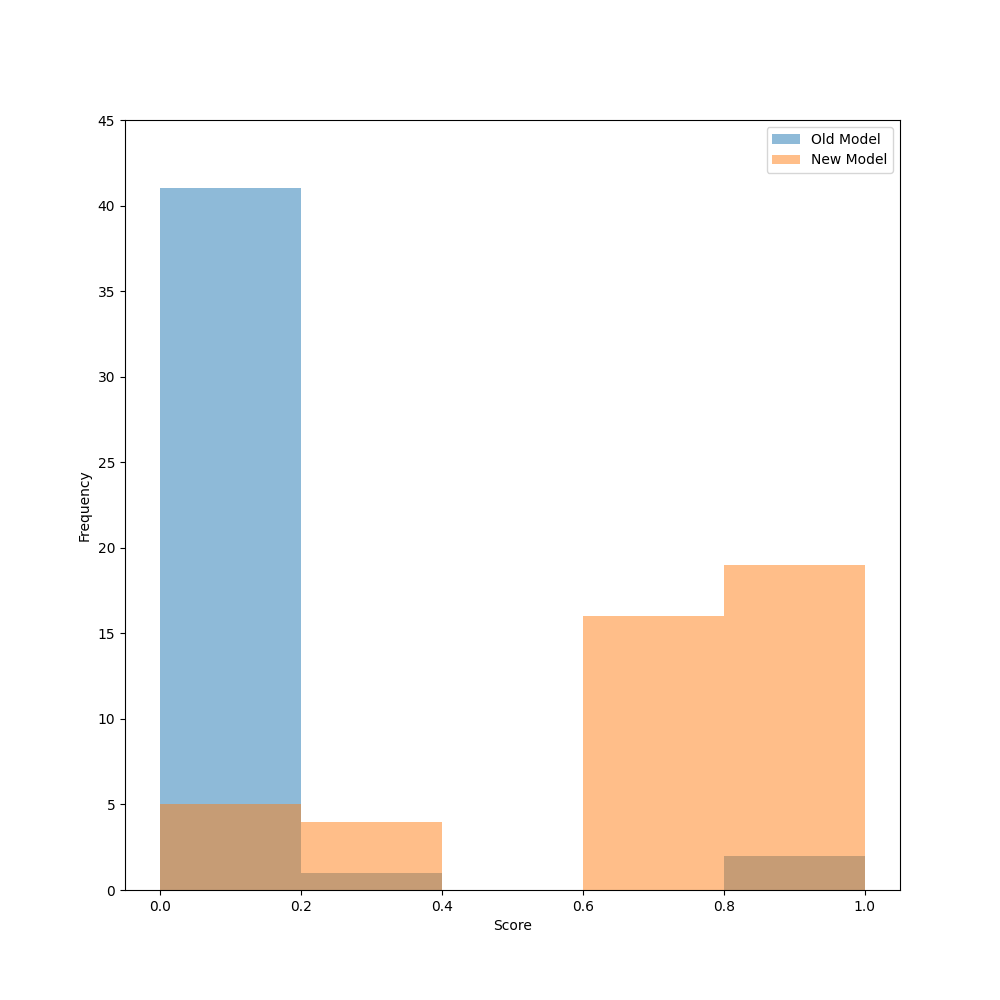
\includegraphics[height=3in, width=3in]{figures/Histogram.png}
\caption{The scorer results in two model }
\label{fig:two model}
\end{figure} 

\subsection{Overall Client-side Content-based Anti-phishing Performance}

As shown in \ref{fig:coverage results}, our experiment demonstrates an important shortcoming about the client-side anti-phishing ecosystem. The phishing websites only became blacklisted if reported; content-based classification and real-time anti-phishing do not contribute to blacklisting.
% \begin{enumerate}
%     \item The websites in groups without reporting did not get blacklisted
%     \item all groups of websites with content-based anti-phishing even with suspicious URLs did not get blacklisted
%     \item The groups of websites with real-time anti-phishing, even with suspicious URLs, did not get blacklisted
% \end{enumerate}
According to the network data files and the crawlers log file, the client-side classifier did not detect these websites as phishing websites. There are two main assumptions for this result:
a)Chrome did not run the classifier on these websites. It might be because avoiding classification when extracting the DOM features takes much time. According to the dynamic analysis of the chromium source code, we found out if extracting DOM elements takes a long time, the classifier runs RunFailure() function and skips the classification.
b)The classifier result score is less than the threshold. This assumption proves the weaknesses of the machine-learning model accuracy.  The client-side content-based anti-phishing accuracy experiment strengthens this assumption.

\subsubsection{Desktop Blacklists}
Our study's primary goal is to identify the effect of client-side content-based anti-phishing on blacklisting newborn phishing websites. After running the main experiment for seven days in mid-may 2020, we analyze the crawler log file and the framework results. Table \ref{fig:coverage results} presents the blacklist coverage for the desktop and mobile google safe browsing blacklists. The key finding in this experiment is the result of the first five groups. For 175 phishing websites, content-based anti-phishing does not affect the blacklisting coverage. For  35 suspicious URLs in group 5, using two client-side anti-phishing methods ( content-based and real-time), there is just one blacklisted phishing URL. The numbers of the blacklisted phishing URL confirm the inefficient performance of google safe browsing client-side anti-phishing methods. The first three groups use the default settings of the chrome browser. 

\subsubsection{Mobile Blacklists}
The majority of Internet traffic users are mobile users~\cite{statcounterglobalstats}, and the earlier study has revealed that mobile web browsers are particularly vulnerable to phishing attacks~\cite{luo2017hindsight}.
We point to one significant finding in our experiment; as shown in table~\ref{fig:coverage results}, none of the phishing sites that used cloaking became blacklist in the mobile chrome browsers while they blacklisted in the desktop chrome browsers. However, the inconsistency between desktop and mobile browsers blacklists of mobile chrome browser previously reported in 2018 by~\cite{oest2019phishfarm}, we showed that this shortcoming still exists.
For mobile chrome browsers with 61.35\%  of all mobile browsers, approximately 2.9 billion users worldwide, this finding is a crucial deficiency in the mobile chrome anti-phishing mechanism.
Although 90\%  of reported websites did blacklist on Desktop Google Safe Browsing, our experiment results showed that 95\%  of all the websites reported to the entities did not blacklist on Mobile Google Safe Browsing~\ref{fig:coverage results}.

\begin{figure*}[t]
  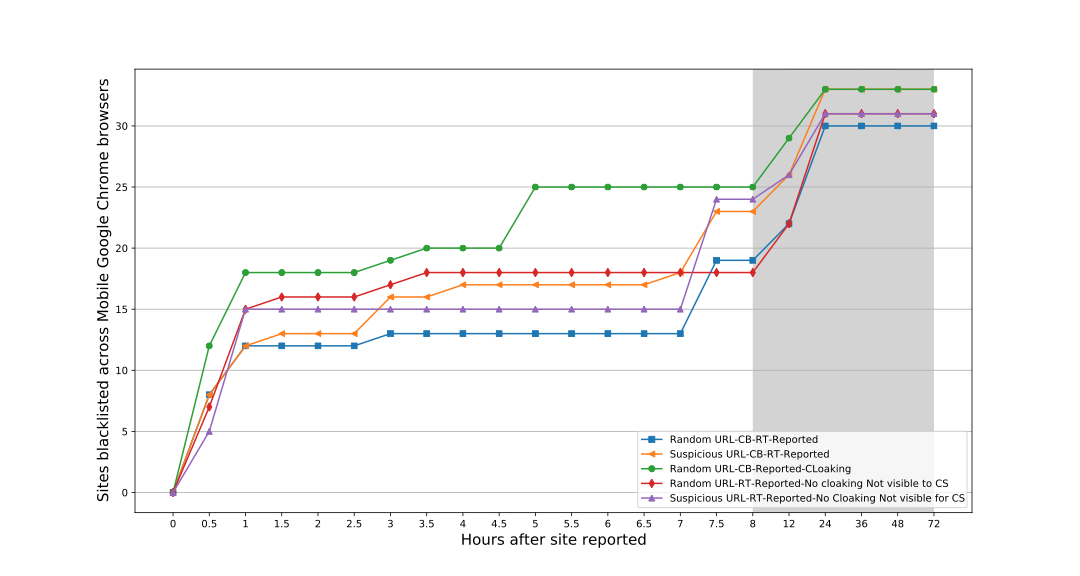
\includegraphics[width=\textwidth,height=9cm]{figures/Mobile-Blacklists-Speed.png}
  \caption{Mobile Blacklisting Performance }
  \label{Blacklisting speed results}
\end{figure*}

% \begin{figure}
%   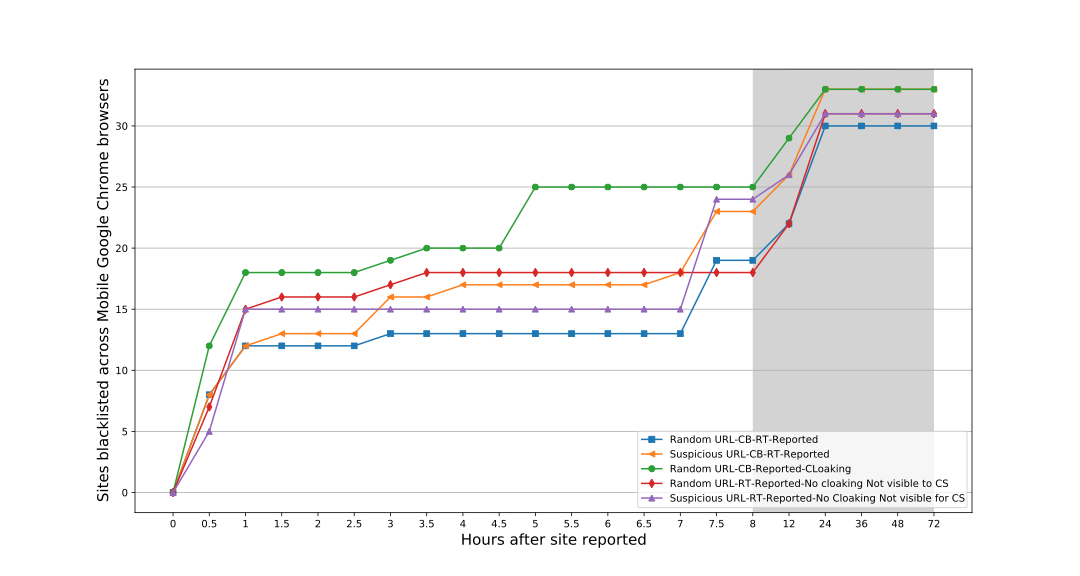
\includegraphics[width=4in,height=3.5in]{figures/Mobile-Blacklists-Speed.png}
%   \caption{Mobile Blacklisting Performance }
%   \label{Blacklisting speed results}
% \end{figure}

%\subsubsection{Long-term Blacklist Consistency} 
\subsection{Blacklist speed}
The main goal of introducing client-side content-based anti-phishing is to cover the 30 minutes gap between updating the local blacklists. The result of our experiment shows that the number of blacklisted phishing websites in the first 30 minutes of the experiment for the not-reported one is zero.
Blacklisting speed for the reported phishing websites is presented in the figure \ref{Blacklisting speed results}. 

\subsection{Real-time anti-phishing evaluation}

Google claims the new real-time anti-phishing 30\%  improves the detection of the un-seen phishing websites. Our experiment results for groups 5 and 6 ( as shown on the table \ref{fig:coverage results} for 70 phishing websites in these two groups, real-time anti-phishing does not affect the blacklisting process as the way it has designed for. For 70 phishing websites, chrome benefits content-based and real-time anti-phishing methods cause blacklisting just one phishing website.

\begin{figure*}[t]
  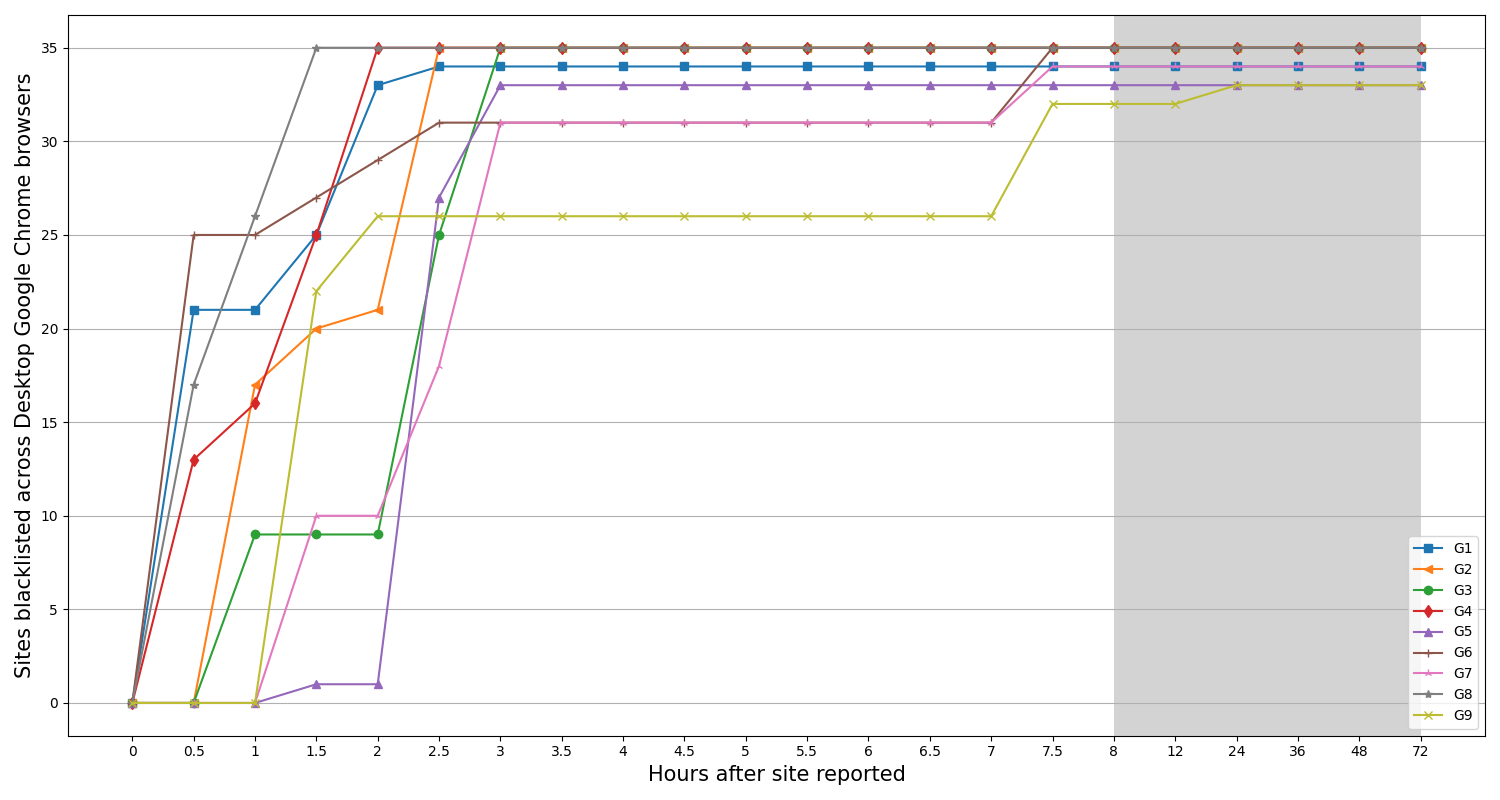
\includegraphics[width=\textwidth,height=9cm]{figures/DesktopBlacklistSpeed.png}
  \caption{Desktop Blacklisting Performance}
  \label{Blacklisting speed results}
\end{figure*}

\subsection{Single-entity Reporting}

Figure \ref{Blacklisting speed results} shows blacklist coverage and speed
for reported phishing websites. In the first 30 minutes, the phishing sites with suspicious URLs, visiting from a browser with active content-based and real-time anti-phishing, and without using cloaking has most blacklisted sites. During the first three of the experiment average, 95\%  of the phishing sites became blacklist regardless of evasion method.
Our study demonstrates that reporting has the most significant role in the blacklisting of un-seen phishing sites.
%add more about content-based to discussion
